\documentclass[9pt]{beamer}
%\usetheme{CambridgeUS}
\usetheme{Antibes}
\usecolortheme[RGB={120,130,235}]{structure}

\usepackage{graphics}
\usepackage{marvosym}
\usepackage{graphicx}
\usepackage{latexsym}
\usepackage{amsmath}
\usepackage{amsfonts,amssymb}
\usepackage{ mathrsfs }
\usepackage{amsthm}
\usepackage{multimedia}
\usepackage{subcaption}
\usepackage{hyperref}
\usepackage{breqn}
\usepackage{wasysym}
\usepackage{xcolor}
\usepackage{ stmaryrd }
\newtheorem{prop}{Proposition}

%Define New Macros
%\input macros
\renewcommand\o{\omega}
\newcommand{\deriv}{\mbox{d}}
\newcommand{\Real}{\mathbb R}
\newcommand{\T}{\mathbb T}
\newcommand{\norm}[1]{\|#1\|}
\newcommand{\abs}[1]{\left\vert#1\right\vert}
\newcommand{\set}[1]{\left\{#1\right\}}
\newcommand{\subheading}[1]{\noindent \textbf{#1}}
\newcommand{\grad}{\nabla}
\newcommand{\diverg}{\textup{div} }
\newcommand{\jump}[1]{[#1]}
\newcommand{\limit}[2]{\lim_{#1 \rightarrow #2}}
\newcommand{\mollify}[1]{ \mathcal{J}_\epsilon #1 }
\newcommand{\conv}[2]{#1 \ast #2}
\newcommand{\D}{D}
\newcommand{\K}{\mathcal{K}}
\newcommand{\ineqtext}[1]{ ^{\text{\tiny #1}}}
\newcommand{\wknorm}[2]{\norm{#1}_{L^{#2,\infty}}}
%\newcommand{\wknorm}[2]{\abs{#1}_{L_w^{#2}}}
\newcommand{\wkspace}[1]{L^{#1,\infty}}
%\newcommand{\wkspace}[1]{L_w^{#1}}
\newcommand{\F}{\mathcal{F}}
\newcommand{\G}{\mathcal{G}}
\newcommand{\eps}{\epsilon}
\newcommand{\lap}{\Delta}

%Nancy's macros
\newcommand{\reg}[1]{#1^\epsilon}
\newcommand{\Lpr}[1]{L^{#1}(\mathbb{R}^n)}
\newcommand{\Lp}[1]{L^{#1}(\Omega)}
\newcommand{\intreal}{\int_{\mathbb{R}^2}\hspace{-8pt}}
\newcommand{\energy}{\mathcal{F}}
\newcommand{\modenergy}{\mathcal{E}_H}
\newcommand{\kernel}{\mathcal{K}}
\newcommand{\into}{\int_{D}}
\newcommand{\intot}{\int_{D_T}}
\newcommand{\ball}{B_n}
\newcommand{\balltime}{B_n\times [0,T]}

\newcommand{\brak}[1]{\langle #1 \rangle} 
\usepackage{url}
\makeatletter
\g@addto@macro{\UrlBreaks}{\UrlOrds}
\makeatother
\newcommand*{\vpointer}{\vcenter{\hbox{\scalebox{2}{\Huge\pointer}}}}


\DeclareMathOperator{\R}{\mathbb{R}}

\title[Proposal Presentation]{Scientific Computation of Two--Phase Ferrofluid Flows} 
\author[Personal Presentation]{Gareth Johnson \\[.3cm] Faculty Adviser: Prof. Ricardo Nochetto } 
\institute[] 
{
	University of Maryland\\ 
	AMSC 663: Advanced Scientific Computing I\\ 
	Supported by Johns Hopkins University Applied Physics Lab
}
\date[October 2018]{October 2, 2018}


\begin{document}
\begin{frame}
	\titlepage
\end{frame}

\section{Introduction}
\begin{frame}{What is a Ferrofluid?}
	\begin{minipage}{.6\paperwidth}
		A ferrofluid is a colloid of nanoscale ferromagnetic particles suspended in a carrier fluid such as oil, water, or an organic solvent.
	\end{minipage}%
	\begin{minipage}{.3\paperwidth}
		\centering
		\flushbottom
		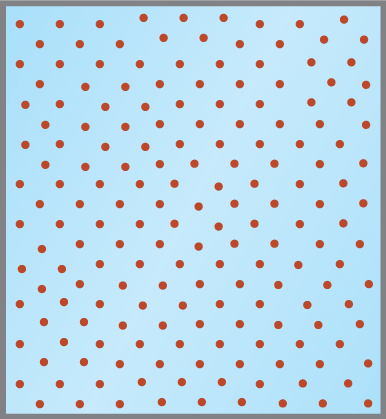
\includegraphics[scale=.5]{Colloid.jpg}
	\end{minipage}%
	\vspace{.3in}\\
	Ferrofluids become magnetized when under the effect of a magnetic field.
	\begin{minipage}{.4\paperwidth}
		\centering
		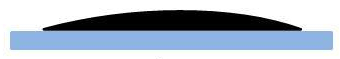
\includegraphics[scale=.3]{FerroStill.jpg}
	\end{minipage}%
	\begin{minipage}{.1\paperwidth}
		$\vpointer$
	\end{minipage}%
	\begin{minipage}{.3\paperwidth}
		\centering
		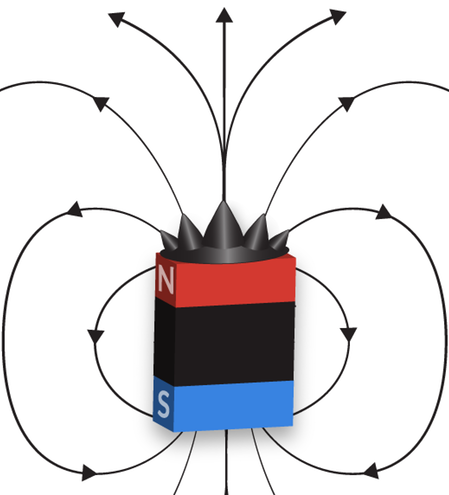
\includegraphics[scale=.18]{FerroExplain.png}
	\end{minipage}
\end{frame}

\begin{frame}{Applications}
	\begin{itemize}
		\item Initially created to pump rocket fuel once a spacecraft entered a weightless environment.
		\begin{minipage}{.5\paperwidth}
			\item Commercial applications:
			\begin{itemize}
				\item Vibration damping
				\item Sensors
				\item Acoustics
			\end{itemize}
			\item Recent research areas:
			\begin{itemize}
				\item Magnetic drug targeting
				\item Adaptive deformable mirrors
			\end{itemize}
		\end{minipage}%
		\begin{minipage}{.3\paperwidth}
			\begin{figure}[!b]
				\centering
				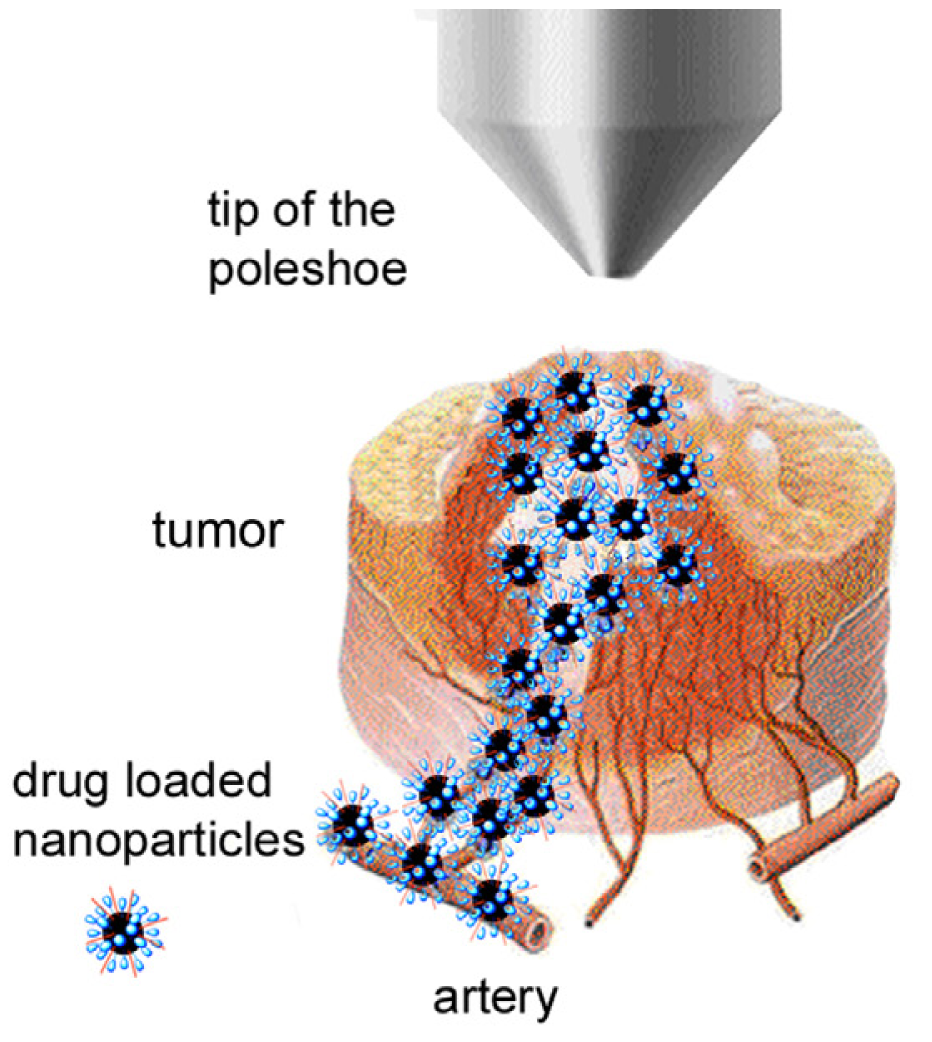
\includegraphics[scale=.7]{DrugTarget.png}
			\end{figure}
		\end{minipage}%
	\end{itemize}
\end{frame}

\begin{frame}{Previous Works}
	\begin{itemize}
		\item Analytic works:
		\begin{itemize}
			\item There are two well established PDE models which mathematically describe the behavior of a ferrofluid under the effects of a magnetic field.
			\begin{itemize}
				\item The Rosensweig model
				\item The Shliomis model 
			\end{itemize}
			\item Existence of global weak solutions and local existence of strong solutions for both models are recent results \cite{PDEResults:1,PDEResults:2, PDEResults:3, PDEResults:4}.
			\item \textcolor{red}{Issue}: There is not an established PDE model which describes two--phase ferrofluid flows.
		\end{itemize}
	
		\item Numerical works:
		\begin{itemize}
			\item Stationary phenomena: Tobiska and collaborators investigated the free surface of ferrofluids using a sharp interface approach.
			\item Non--stationary phenomena: Using a Volume of Fluid method
			\begin{itemize}
				\item  the field induced motion of a ferrofluid droplet was investigated \cite{Numerics:1},
				\item  the formation of ferrofluid droplets was investigated \cite{Numerics:2}.
			\end{itemize}
			\item \textcolor{red}{Issue}:The above techniques numerical implementations, stability, and convergence were not explored.
		\end{itemize}
	\end{itemize}
\end{frame}

\section{PDE Model for Two--Phase Ferrofluid Flows}
\begin{frame}{PDE Model for Two--Phase Ferrofluid Flow}
	\begin{itemize}
		\item Dr. Nochetto and collaborators developed a model for two--phase ferrofluid flows and devised an energy stable numerical scheme \cite{DiffuseInterface}.
		\vspace{.1in}
		\item The model was not derived, but instead was assembled.
		\vspace{.1in}
		\item Important results from \cite{DiffuseInterface}:
		\begin{itemize}
			\item Proved an energy law for the PDE model.
			\item Proved the numerical scheme was energy stable and the existence of a local solution.
			\item For an even simpler model, they proved stability, convergence, and the existence of solutions.
		\end{itemize}
	\end{itemize}
\end{frame}

\subsection{Cahn--Hilliard Equation}
\begin{frame}{Modeling a Two--Phase Fluid}
\begin{itemize}
	\item In order to track both fluids, a diffuse interface is used.
	\item The phase variable $\theta$ is introduced, which takes values in $[-1,1]$.
	\item The evolution of $\theta$ is given by a modified Cahn--Hilliard equation:
	\vspace{.1in}\\
	\begin{minipage}{.5\paperwidth}
		$$
		\left\{
		\begin{aligned}
		\theta_t + \diverg(\mathbf{u}\theta) + \gamma \lap \psi &= 0 &\text{in }\Omega \\
		\psi - \eps \lap \theta + \frac{1}{\eps}f(\theta) &= 0 & \text{in }\Omega \\
		\partial_\eta \theta = \partial_\eta\psi &= 0 & \text{on }\Gamma,
		\end{aligned}
		\right.
		$$
		where
		\begin{itemize}
			\item $0 < \eps << 1$ is related to the interface thickness,
			\item $\gamma >0$ is the constant mobility,
			\item $\psi$ is the chemical potential,
			\item $f(\theta)$ is the truncated double well potential.
		\end{itemize}
	\end{minipage}%
	\begin{minipage}{.3\paperwidth}
		\begin{figure}[!b]
			\centering
			
			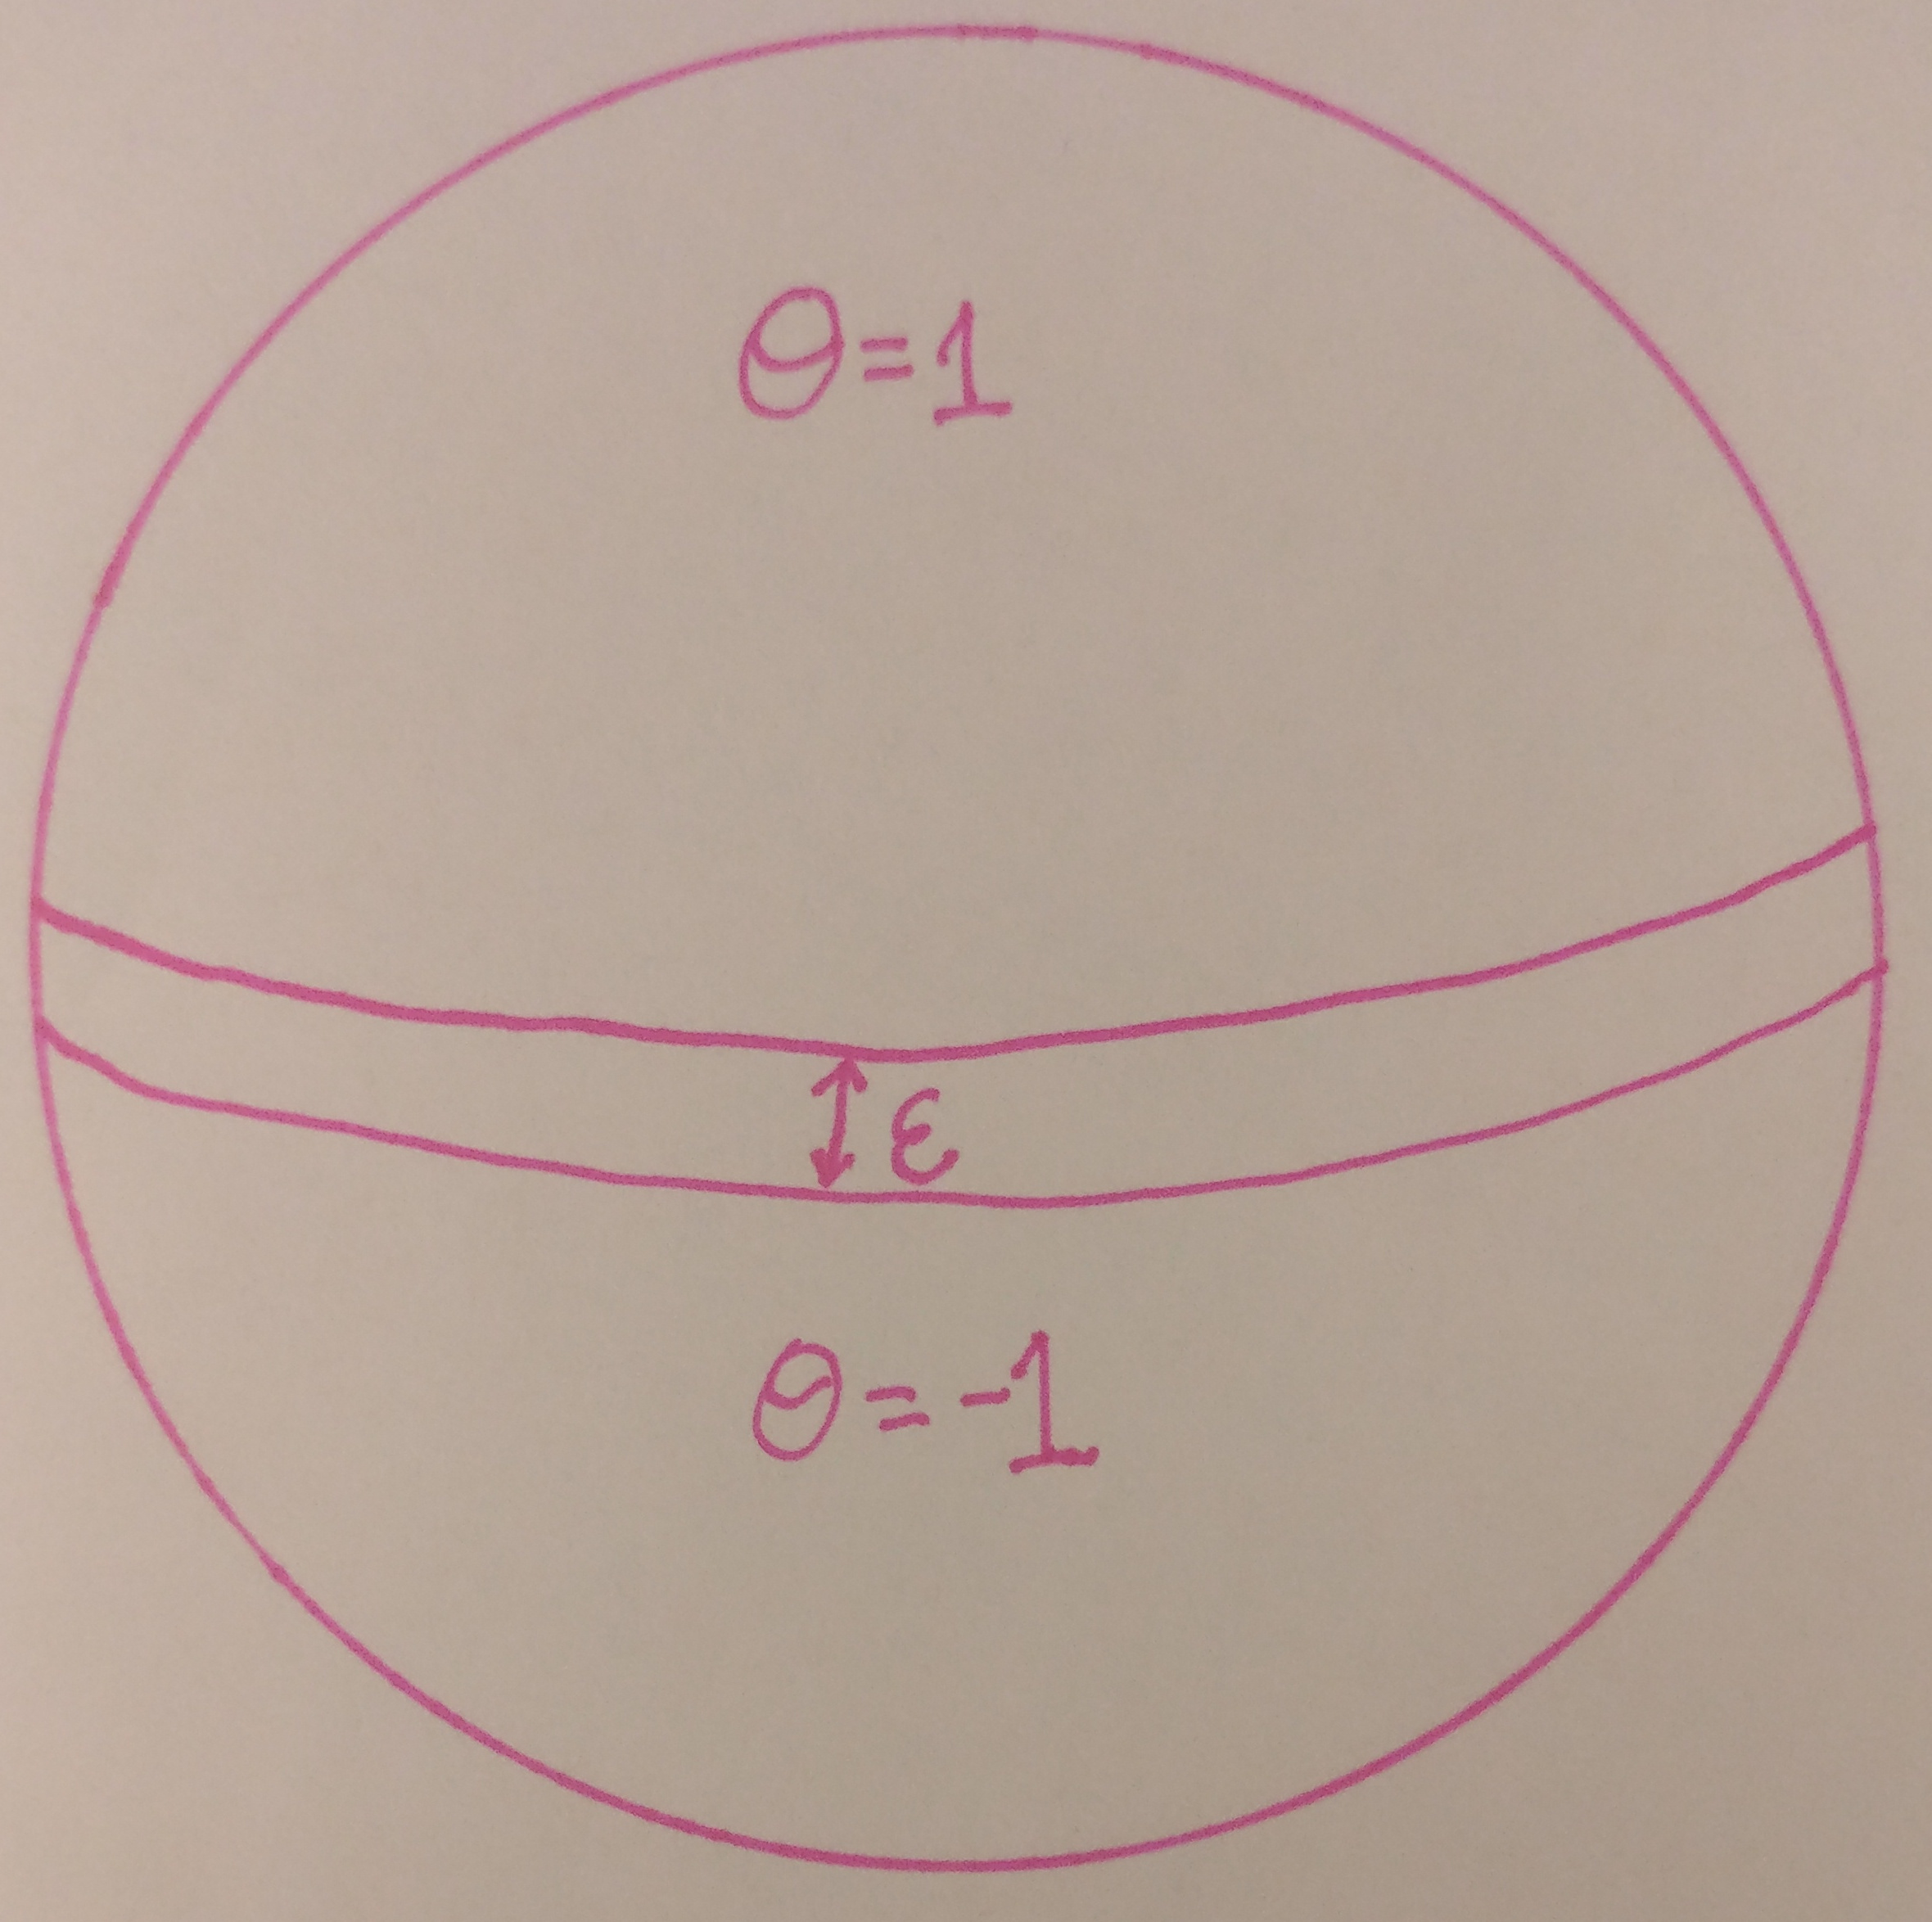
\includegraphics[scale=.05]{CahnHilliard.jpg}
		\end{figure}
	\end{minipage}%
\end{itemize}
\end{frame}

\subsection{Magnetic Field Equations}
\begin{frame}{Modeling of the Magnetic Field}
\begin{itemize}
	\item Instead of using the magnetostatics equations, a simplified approach was used.
	\item Define the magnetic field by 
	$$
		\mathbf{h} := \mathbf{h}_a + \mathbf{h}_d,
	$$
	where 
	\begin{itemize}
		\item $\mathbf{h}_a$ -- smooth harmonic (curl--free and $\diverg$--free) applied magnetizing field,
		\item $\mathbf{h}_d$ -- demagnetizing field.
	\end{itemize}
	\item Then the magnetic field is induced via the scalar potential $\varphi$ by
	$$
		\mathbf{h} = \grad\varphi,
	$$
	along with,
	$$
		-\lap \varphi =\diverg(\mathbf{m}-\mathbf{h}_a) \quad \text{in }\Omega,\quad \quad \partial_\eta\varphi = (\mathbf{h}_a - \mathbf{m})\cdot\eta \quad \text{on }\Gamma.
	$$
\end{itemize}
\end{frame}

\subsection{Ferrohydrodynamics Equations}
\begin{frame}{Modeling of Ferrohydrodynamics}
\begin{itemize}
	\item A simplified version of Shliomis model is used, which couples an advection--reaction equation for the magnetization $\mathbf{m}$:
	$$
		\mathbf{m}_t + (\mathbf{u}\cdot \grad)\mathbf{m}=-\frac{1}{\mathscr{T}}(\mathbf{m} - \varkappa_\theta\mathbf{h}),
	$$
	with the Navier--Stokes equations of incompressible fluids for the velocity--pressure pair $(\mathbf{u},p)$:
	\begin{align*}
		\mathbf{u}_t + (\mathbf{u}\cdot\grad)\mathbf{u} - \diverg (\nu_\theta \mathbf{T(u)}) + \grad p &= \mu_0(\mathbf{m}\cdot \grad)\mathbf{h} + \frac{\lambda}{\eps}\theta\grad \psi,\\
		\diverg \mathbf{u} &= 0,
	\end{align*}
	where
	\begin{itemize}
		\item $\mathscr{T}$ is the relaxation time of the ferrofluid,
		\item $\varkappa_\theta$ is the magnetic susceptibility of the phase variable,
		\item $\nu_\theta$ is the viscosity of the phase variable,
		\item $\mu_0$ is the constitutive parameter related to the Kelvin force,
		\item $\frac{\lambda}{\eps}\theta\grad \psi$ is the capillary force.
	\end{itemize}
	\item This is supplemented with a no--slip condition on the boundary:
	$$
		\mathbf{u} = 0 \quad \text{on }\Gamma. 
	$$
\end{itemize}
\end{frame}

\subsection{Full Model}
\begin{frame}
\begin{itemize}
	\item The model reads: Consider a bounded convex polygon/polyhedron domain $\Omega\subset \Real^d$ ($d=2$ or $3$) with boundary $\Gamma$. The evolution of the system is given by the following set of equations in strong form in $\Omega$
	\begin{subequations}\label{Model}
		\begin{align}
		\label{Cahn-Hilliard:1}\theta_t + \diverg(\mathbf{u}\theta) + \gamma \lap \psi &= 0,\\
		\label{Cahn-Hilliard:2}\psi - \eps \lap \theta + \frac{1}{\eps}f(\theta) &= 0,\\
		\label{Advection-Reaction}\mathbf{m}_t + (\mathbf{u}\cdot \grad)\mathbf{m}&=-\frac{1}{\mathscr{T}}(\mathbf{m} - \varkappa_\theta\mathbf{h}),\\
		\label{MagScalarPot}-\lap \varphi &=\diverg(\mathbf{m}-\mathbf{h}_a),\\
		\label{NavierStokes}\mathbf{u}_t + (\mathbf{u}\cdot\grad)\mathbf{u} - \diverg (\nu_\theta \mathbf{T(u)}) + \grad p &= \mu_0(\mathbf{m}\cdot \grad)\mathbf{h} + \frac{\lambda}{\eps}\theta\grad \psi,\\
		\label{DivFree}\diverg \mathbf{u} &= 0,
		\end{align}
	\end{subequations}
	for every $t\in[0,t_F]$, where $\mathbf{T(u)}=\frac{1}{2}(\grad \mathbf{u} + \grad\mathbf{u}^T)$ denotes the symmetric gradient and $\mathbf{h}=\grad \varphi$. The system (\ref{Model}) is supplemented with the boundary conditions
	\begin{equation}\label{ModelBC}
	\partial_\eta \theta = \partial_\eta\psi = 0,\quad \mathbf{u}=0,\quad\text{and}\quad \partial_\eta\varphi = (\mathbf{h}_a - \mathbf{m})\cdot\eta \quad \text{on }\Gamma.
	\end{equation}
\end{itemize}
\end{frame}

\section{Numerical Method}
\begin{frame}
	Define the backward difference operator $\delta f^k = f^k - f^{k-1}$.\\
	\vspace{.1in}
	For given smooth initial data $\set{\Theta^0, \mathbf{M}^0,\mathbf{U}^0}$ and timestep $\tau$, compute $\set{\Theta^k, \Psi^k, \mathbf{M}^k, \Phi^k, \mathbf{U}^k, {P}^k}\in \mathbb{G}_h\times \mathbb{Y}_h\times \mathbb{M}_h\times\mathbb{X}_h\times\mathbb{U}_h\times\mathbb{P}_h$ for every $k\in\set{1,...,K}$ that solves
	
	\footnotesize\begin{subequations}\label{NumScheme}
		\begin{align}
		\label{NumScheme:1}\bigg(\frac{\delta\Theta^k}{\tau}, \Lambda\bigg) - (\mathbf{U}^k\Theta^{k-1}, \grad\Lambda) - \gamma(\grad \Psi^k, \grad \Lambda)&=0,\\
		\label{NumScheme:2}(\Psi^k, \Upsilon) + \eps(\grad \Theta^k, \grad \Upsilon) + \frac{1}{\eps}(f(\Theta^{k-1}), \Upsilon) + \frac{1}{\eta}(\delta\Theta^k, \Upsilon) &= 0,\\
		\label{NumScheme:3}\bigg(\frac{\delta\mathbf{M}^k}{\tau}, \mathbf{Z}\bigg) - \mathcal{B}_h^m(\mathbf{U}^k, \mathbf{Z}, \mathbf{M}^k) + \frac{1}{\mathscr{T}}(\mathbf{M}^k, \mathbf{Z}) &= \frac{1}{\mathscr{T}}(\varkappa_\theta\mathbf{H}^k, \mathbf{Z}),\\
		\label{NumScheme:4}(\grad\Phi^k, \grad X) &= (\mathbf{h}_a^k - \mathbf{M}^k, \grad X),\\
		\begin{split}
		\label{NumScheme:5}\bigg(\frac{\delta\mathbf{U}^k}{\tau}, \mathbf{V}\bigg) + \mathcal{B}_h(\mathbf{U}^{k-1}, \mathbf{U}^k, \mathbf{V}) + (\nu_\theta\mathbf{T(U}^k), \mathbf{T(V)}) - (P^k, \diverg \mathbf{V}) &= \mu_0\mathcal{B}_h^m(\mathbf{V}, \mathbf{H}^k, \mathbf{M}^k)\\
		&\phantom{{}={}}+\frac{\lambda}{\eps}(\Theta^{k-1}\grad \Psi^k, \mathbf{V}),
		\end{split}\\
		\label{NumScheme:6}(Q, \diverg\mathbf{U}^k) &= 0.
		\end{align}
	\end{subequations}
	\normalsize
\end{frame}

\section{Project Goals}
\begin{frame}{Project Goals}
	\begin{itemize}
		\item[1)] Finite Element Code: Develop a finite element code to solve two--phase ferrofluid flows using the numerical scheme (\ref{NumScheme}). This code will be written in a ``dimensional--less" way, explained later, so that the code can be easily transitioned from 2d to 3d.
		
		\item[2)] Solvers: In order to solve (\ref{NumScheme}), three different solvers are required.
		
		\item[3)] Scientific Questions: Investigate the structure of the velocity field of the fluid flow and the and magnetic field around the spike deformation of the ferrofluid for both the Rosenswieg instability and the ferrofluid hedgehog configuration in 2d.
	\end{itemize}
	If time permits, the following extensions of the project will be explored:
	\begin{itemize}
		\item[4)] Parallelization: Implement parallel adaptive mesh refinement/coarsening.
		
		\item[5)] Ferrofluid Droplets: Investigate if the model can accurately capture various effects of ferrofluid droplets, such as the coalescence of droplets \cite{CompDropplet} and the equilibrium shape of droplets under a uniform magnetic field \cite{DroppletDeform}.
	\end{itemize}
\end{frame}

\section{Approach}
\begin{frame}
\section{Approach}
Finite Element Code:
\begin{itemize}
	\item[1)] Write codes to handle the generation of the finite element spaces given in \cite{DiffuseInterface}. 
	
	\item[2)] Write codes to handle the generation and adaptive refinement/coarsening of the mesh.
	
	\item[3)] Write a code to handle the generation of the matrices, which will combine information from the mesh and the finite elements. 
	
	\item[4)] Write codes that solve each of the three subsystems, namely the Cahn--Hilliard system (\ref{NumScheme:1})--(\ref{NumScheme:2}), the magnetization system (\ref{NumScheme:3})--(\ref{NumScheme:4}), and the Navier--Stokes system (\ref{NumScheme:5})--(\ref{NumScheme:6}).
	
	\item[5)] Write a code to solve the full system (\ref{NumScheme}) at each time step using a Picard--like iteration.
	
	\item[6)] Write a code to handle the generation of the magnetic potential, given the locations of each magnetic dipole.
	
	\item[7)] Include functionality for the numerical simulation to be restarted from the last completed iteration.
\end{itemize}
Numerical Investigation:
\begin{itemize}
	\item Generate and analyze contour and vector plots of the velocity and magnetic field for the three experiments performed in \cite{DiffuseInterface}.
\end{itemize}
\end{frame}

\section{Numerical Implementation}
\begin{frame}{Discretization of the Numerical Scheme}
	Recall (\ref{NumScheme}):
	\footnotesize\begin{align*}
		\bigg(\frac{\delta\Theta^k}{\tau}, \Lambda\bigg) - (\mathbf{U}^k\Theta^{k-1}, \grad\Lambda) - \gamma(\grad \Psi^k, \grad \Lambda)&=0,\\
		(\Psi^k, \Upsilon) + \eps(\grad \Theta^k, \grad \Upsilon) + \frac{1}{\eps}(f(\Theta^{k-1}), \Upsilon) + \frac{1}{\eta}(\delta\Theta^k, \Upsilon) &= 0,\\
		\bigg(\frac{\delta\mathbf{M}^k}{\tau}, \mathbf{Z}\bigg) - \mathcal{B}_h^m(\mathbf{U}^k, \mathbf{Z}, \mathbf{M}^k) + \frac{1}{\mathscr{T}}(\mathbf{M}^k, \mathbf{Z}) &= \frac{1}{\mathscr{T}}(\varkappa_\theta\mathbf{H}^k, \mathbf{Z}),\\
		(\grad\Phi^k, \grad X) &= (\mathbf{h}_a^k - \mathbf{M}^k, \grad X),\\
		\begin{split}
		\bigg(\frac{\delta\mathbf{U}^k}{\tau}, \mathbf{V}\bigg) + \mathcal{B}_h(\mathbf{U}^{k-1}, \mathbf{U}^k, \mathbf{V}) + (\nu_\theta\mathbf{T(U}^k), \mathbf{T(V)}) - (P^k, \diverg \mathbf{V}) &= \mu_0\mathcal{B}_h^m(\mathbf{V}, \mathbf{H}^k, \mathbf{M}^k)\\
		&\phantom{{}={}}+\frac{\lambda}{\eps}(\Theta^{k-1}\grad \Psi^k, \mathbf{V}),
		\end{split}\\
		(Q, \diverg\mathbf{U}^k) &= 0.
	\end{align*}
	\begin{itemize}
		\item Time Discretization: Backward Euler is used.
		\item Space Discretization: A mix of Continuous and Discontinuous Galerkin is used, approximating the spaces with polynomials of degree $2$ in each variable.
		\begin{itemize}
			\item Continuous: Cahn--Hilliard and Navier Stokes equations.
			\item Discontinuous: Magnetization equations.
		\end{itemize}
	\end{itemize}
\end{frame}

\begin{frame}{Fixed Point Solver}
	\begin{itemize}
		\item A Picard--like iteration is used.
		\item Utilizes the "lagging" of the velocity $\mathbf{U}$ to solve each subsystem.
		\item Iterates until a fixed point for $\mathbf{U}^k$ is reached.
	\end{itemize}
	\vspace{.2in}
	Given $\mathbf{U}^{k-1}$ 
	\begin{itemize}
		\item[1)] Compute $\Theta^k$ and $\Psi^k$ substituting $\mathbf{U}^{k-1}$ for $\mathbf{U}^{k}$.
		
		\item[2)] Next compute $\mathbf{M}^k$ and $\Phi^k$ using $(\Theta^k,\Psi^k)$ from the previous iteration and substituting $\mathbf{U}^{k-1}$ for $\mathbf{U}^{k}$.
		
		\item[3)] Finally, compute $\mathbf{U}^k$ and $P^k$ using $(\Theta^k,\Psi^k, \mathbf{M}^k, \Phi^k)$ from the previous two iterations.
		
		\item[4)] Repeat steps 1-3 using $\mathbf{U}^k$ from the previous iteration as input until $\mathbf{U}^k$ does not change between iterations.
	\end{itemize}
\end{frame}

\begin{frame}{Subsystem Solvers}
	Cahn--Hilliard system (\ref{NumScheme:1})--(\ref{NumScheme:2}):
	\begin{itemize}
		\item Linearized using convex--concave splitting:
		$$
			f(\Theta^k)\to f(\Theta^{k-1}) + \eta \delta \Theta^k, \quad \quad \text{where } \eta\leq \big(\max_\theta f'(\theta)\big)^{-1}.
		$$
		\item The resulting system is linear but non--symmetric.
		\item Solved using GMRES preconditioned with algebraic multigrid.
	\end{itemize}
	Magnetization system (\ref{NumScheme:3})--(\ref{NumScheme:4}):
	\begin{itemize}
		\item Equation (\ref{NumScheme:3}) is mass dominated and non--symmetric.
		\item Solved using BiCGstab.
		\item Equation (\ref{NumScheme:4}) is a Laplacian, which is symmetric.
		\item Solved using CG preconditioned with algebraic multigrid.
	\end{itemize}

	Navier--Stokes system (\ref{NumScheme:5})--(\ref{NumScheme:6}):
	\begin{itemize}
		\item It is a non--symmetric saddle point problem.
		\item Solved using GMRES with a block preconditioner.
		\item Will explore preconditioners presented in Elman's book \cite{Precond}.
	\end{itemize}
\end{frame}

\begin{frame}{Adaptive Mesh Refinement/Coarsening}
	\begin{itemize}
		\item In order to resolve the interface, we need $0 < \eps << 1$.
		\item This requires the mesh to be highly dense near the interface.
		\item If a uniform meshsize $h$ is used, this would lead to very large linear systems.
		\item To overcome this, we will use adaptive mesh refinement/coarsening.
		\begin{figure}[!ht]
			\centering
			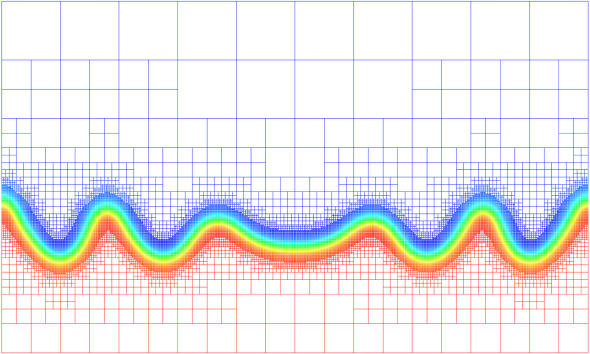
\includegraphics[scale=.4]{Mesh.jpg}
		\end{figure}
		\item The adaptive mesh refinement/coarsening will use the simplest element indicator $\eta_T$:
		$$
			\eta_T^2 = h_T\int_{\partial T}\abs{\bigg\llbracket\frac{\partial \Theta}{\partial \eta}\bigg\rrbracket}^2dS \quad \forall T\in\mathcal{T}_h.
		$$
	\end{itemize}
\end{frame}

\begin{frame}{Generation of the Magnetic Field}
	\begin{minipage}{.6\paperwidth}
		Define the magnetic dipole $\phi_s$ by
		$$
		\phi_s(\mathbf{x}) = \frac{\mathbf{d}\cdot(\mathbf{x}_s - \mathbf{x})}{\abs{\mathbf{x}_s - \mathbf{x}}}, 
		$$
		where $\abs{\mathbf{d}}=1$ and $\mathbf{d},\mathbf{x}_s,\mathbf{x}\in\Real^2$. Then the applied\\ magnetizing field $\mathbf{h}_a$ is given by
		$$
		\mathbf{h}_a = \sum_s \alpha_s(t) \grad\phi_s,
		$$
		where $\alpha_s(t)$ is the intensity of each dipole.
	\end{minipage}%
	\begin{minipage}{.3\paperwidth}
		\begin{figure}[!b]
			\centering
			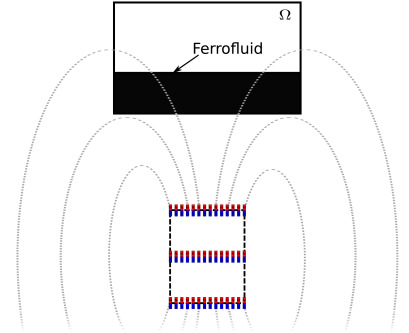
\includegraphics[scale=.4]{MagField.jpg}
		\end{figure}
	\end{minipage}%
\end{frame}

\section{Implementation Details}
\begin{frame}{Target Platform}
	Hardware:
	\begin{itemize}
		\item A Linux desktop system.
	
		
		\item Using desktop owned by Dr. Nochetto with a Intel Xeon CPU with 24 cores and 68 GB of ram
	\end{itemize}

	Software:
	\begin{itemize}
		\item Developed in C++.
		
		\item The code will utilize the deal.II library \cite{AdaptiveMesh:1,DealII}. The library provides functionality to
		\begin{itemize}
			\item create meshes,
			\item generate finite elements,
			\item aid in adaptive mesh refinement/coarsening,
			\item solve linear algebra systems with preconditioners.
		\end{itemize}
	\end{itemize}

	Distribution:
	\begin{itemize}
		\item Source code and user guide will be hosted on Github.
	\end{itemize}
\end{frame}

\section{Validation}
\begin{frame}{Validation Methods}
	Generated Solutions:
	\begin{itemize}
		\item Each of the three subsystems will be verified using a generated solution.
		\item Simple Example: For $u=\sin(x)$ to be a solution to 
		$$
			u' + u = 0,
		$$
		the forcing $f(x) = \sin(x) + \cos(x)$ will be added to the RHS.
	\end{itemize}
	
	Mesh Verification:
	\begin{itemize}
		\item Visually will verify input mesh.
		
		\item Adaptive mesh refinement/coarsening verified using a simple mesh with assigned error values.
	\end{itemize}
\end{frame}

\begin{frame}{Verification Methods (continued)}
	Comparison with prior works:
	\begin{minipage}{.3\paperwidth}
		\begin{figure}[!b]
			\centering
			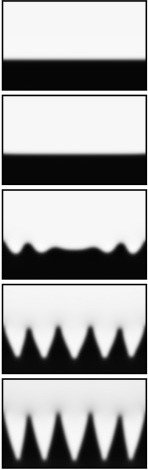
\includegraphics[scale=.56]{Instab.jpg}
			\caption*{Uniform Magnetic Field}
		\end{figure}
	\end{minipage}%
	\begin{minipage}{.3\paperwidth}
		\begin{figure}[!b]
			\centering
			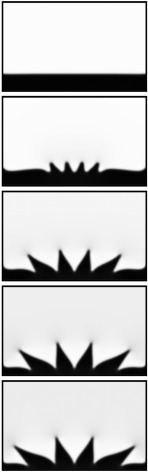
\includegraphics[scale=.56]{Hedgehog.jpg}
			\caption*{Non--uniform magnetic field\\ \centering$\mathbf{h} := \mathbf{h}_a + \mathbf{h}_d$}
		\end{figure}
	\end{minipage}%
	\begin{minipage}{.3\paperwidth}
		\begin{figure}[!b]
			\centering
			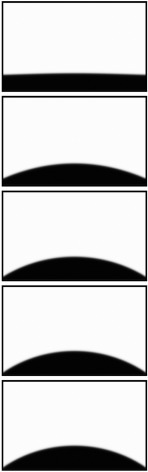
\includegraphics[scale=.56]{Oval.jpg}
			\caption*{Non--uniform magnetic field\\ \centering$\mathbf{h} := \mathbf{h}_a$}
		\end{figure}
	\end{minipage}%
\end{frame}

\section{References}
\begin{frame}{Figure References}
\begin{itemize}
	\item Slide 1:
	\begin{itemize}
		\item \url{https://www.researchgate.net/profile/Vikram\_Raghavan2/post/What\_is\_the\_effect\_of\_magnetic\_field\_on\_alignment\_of\_ferro\_fluid\_droplet/attachment/59d622166cda7b8083a1b9a2/AS\%3A273810673078272\%401442292959057/download/Effect+of+Magnetic+field.jpg}
		\item \url{https://ksr-ugc.imgix.net/assets/003/310/641/f0ef73d1fd99f6aa5d96872168478df4\_original.png?v=1424378871\&w=680\&fit=max\&auto=format\&lossless=true\&s=c183d857603c12de82a71f3139283d9e}
		\item \url{https://opentextbc.ca/chemistry/wp-content/uploads/sites/150/2016/05/CNX\_Che\_11\_05\_Colloid.jpg}
	\end{itemize}
	\item Slide 2: \cite{DrugTarget}
	\item Slide 15: \cite{DiffuseInterface}
	\item Slide 16: \cite{DiffuseInterface}
	\item Slide 18: \cite{DiffuseInterface}
\end{itemize}
\end{frame}

\tiny

\begin{frame}[allowframebreaks]{References}
	\bibliographystyle{siam}
	\bibliography{ProposalPresentation}
\end{frame}




\end{document}
